\section{Results: MRI in self-gravitating disks}

\subsection{Influence of self-gravity on the MRI through the
  background equilibrium}
 
In this section we focus on the MRI. We consider polytropic disks,
which have a well-defined thickness, and a vertical field. 
We set the upper disk boundary at $Z_s=0.99H$ and fix $\beta=100$ and
$k_xH=0.1$. The numerical resolution is $N_z=256$.  

%kx -> 0 so incompressible 

\subsubsection{Uniform
  resistivity}  
We first calculate the MRI as a function of $Q$ with uniform
resistivity ($A=1$) for mid-plane Elsasser numbers $\Lambda_0\in[0.3,10]$.    

Fig. \ref{compare_growth_poly_uniresis} plots the MRI growth rates as
a function of $Q$ and $\Lambda_0$. As expected growth rates generally
decrease with increasing $\Lambda_0$. In the limit of ideal MHD ($\Lambda_0>1$), 
there is negligible dependence on $Q$. In the resistive limit
($\Lambda_0<1$), however, growth rates decrease noticeably for $Q<1$. This shows
show that disk self-gravity affects the MRI through the background
equilibrium, even though density and potential perturbations are  
negligible (i.e. the linear response is
non-self-gravitating).    
 
\begin{figure}
  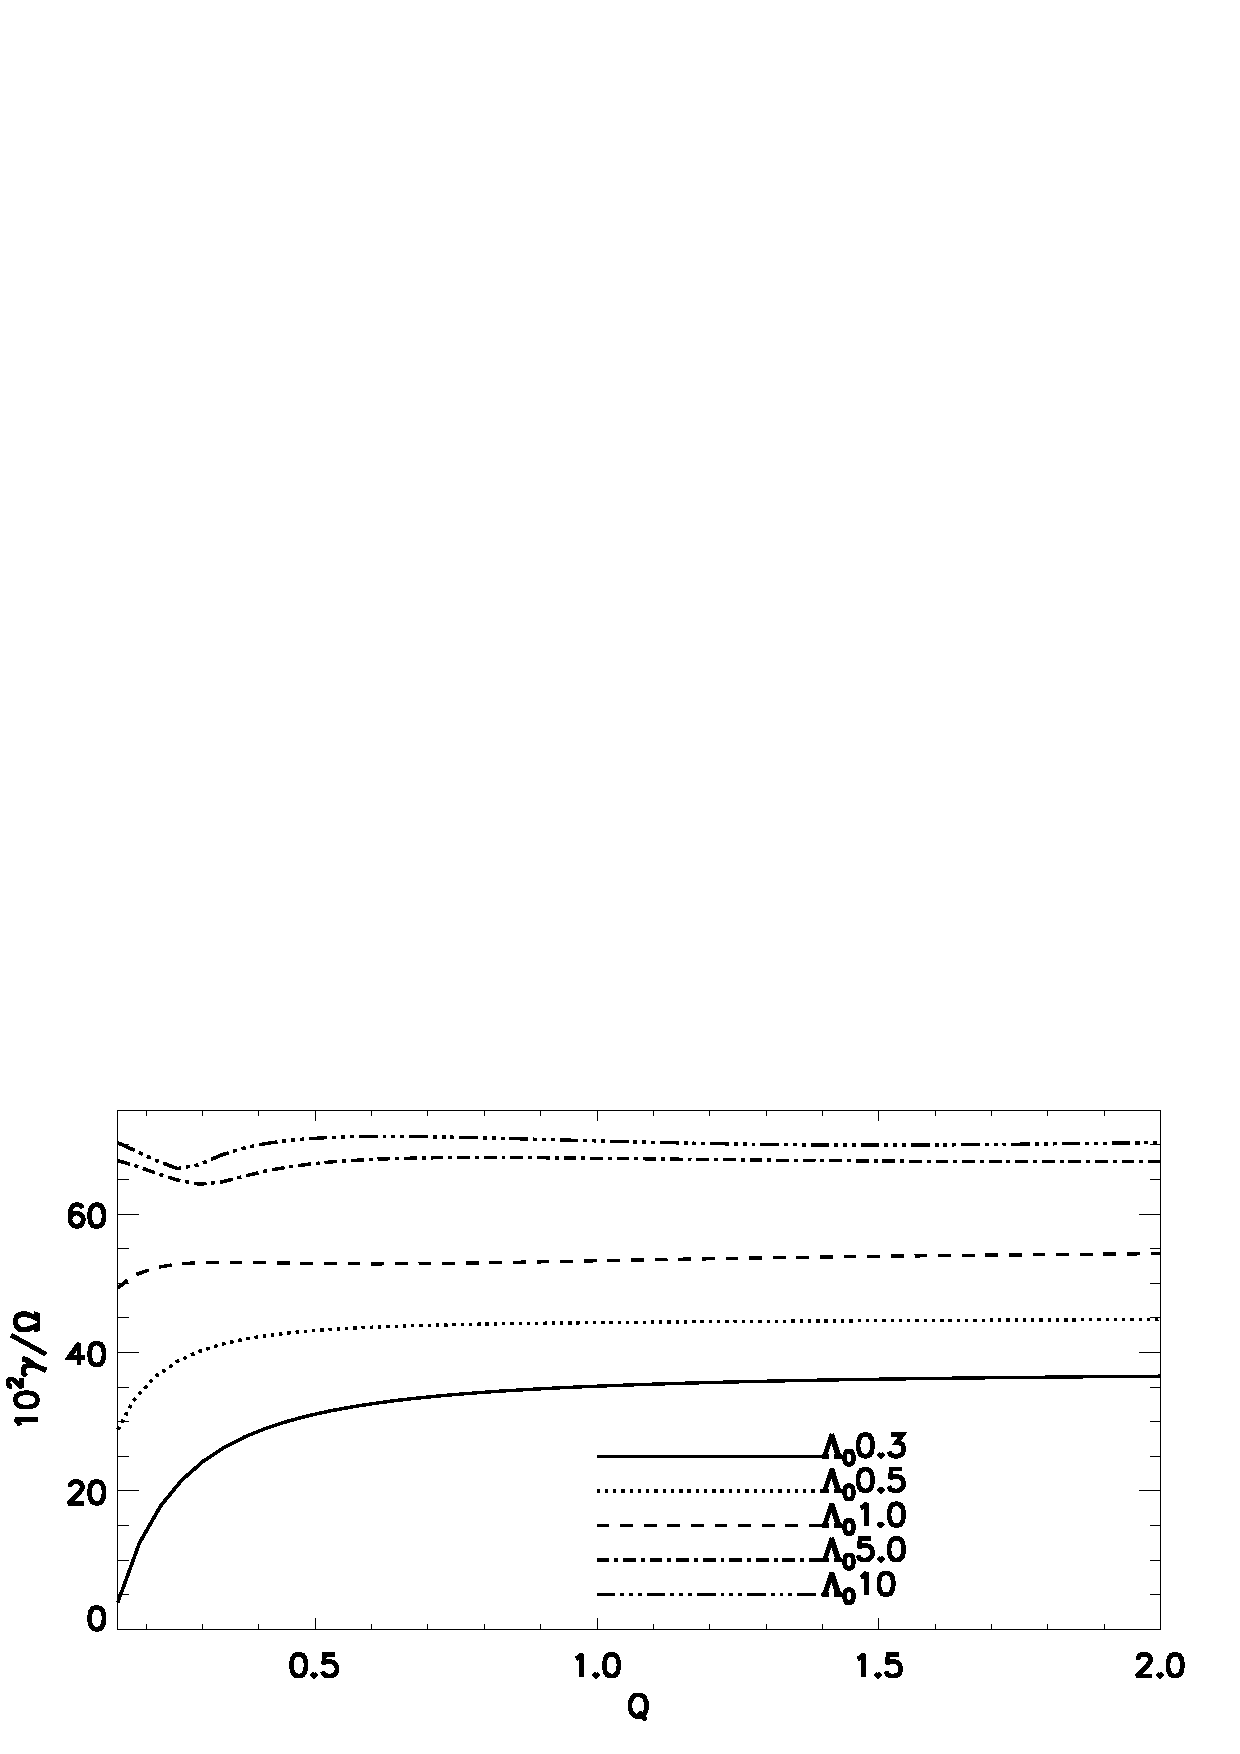
\includegraphics[width=\linewidth]{figures/compare_growth_poly_uniresis2}
  \caption{MRI growth rates as a function of $Q$ for mid-planet
    Elsasser numbers $\Lambda_0=0.3$ (solid), $0.5$ (dotted), $1.0$
    (dashed) and $5.0$ (dash-dot).  
    \label{compare_growth_poly_uniresis}}
\end{figure}

\cite{sano99} found that for instability to occur the linear mode
wavelength $\lambda$ should fit inside the disk. That is,   
\begin{align}\label{sano_crit}
  \lambda \equiv
  \mathrm{max}\left(\lambda_\mathrm{ideal},\lambda_\mathrm{resis}\right)\lesssim
  2H, 
\end{align}
where the MRI wavelengths are given by 
\begin{align}\label{lambda_ideal}
  \frac{\lambda_\mathrm{ideal}}{2H} = \frac{4\pi}{\sqrt{15}} f \hat{v}_A =
  \frac{4\pi f}{\sqrt{15\beta\hat{\rho}}}
\end{align}
in the limit of ideal MHD, and 
\begin{align}\label{lambda_resis}
  \frac{\lambda_\mathrm{resis}}{2H} = \frac{2\pi}{\sqrt{3}}\frac{\hat{\eta}}{\hat{v}_A f} =
  \frac{2\pi f}{\Lambda_0}\sqrt{\frac{\hat{\rho}}{3\beta}} 
\end{align}
in the limit of high resistivity.  
   
Since $\hat{\rho}$ is weakly dependent
on $Q$ (Fig. \ref{eqm_den}), self-gravity only affects the
MRI through the factor $f$, which increases with decreasing $Q$ (see
Fig. \ref{plot_fq} in Appendix \ref{appen1}). This suggests that
sufficiently strong self-gravity can stabilize the MRI by making
$ 2H<\lambda $. 
 

In the ideal limit, we find $\lambda < 2H$ throughout most of the disk
for the values of $Q$ considered, so that self-gravity does not affect
growth rates significantly. However, the wavelength of the instability
increases. This is shown in Fig. \ref{compare_result_lambda10} which
plots the magnetic energies for $\Lambda_0=10$ and a range of Toomre $Q$
values. The number of vertical nodes decrease with $Q$, 
i.e. the disk accommodates fewer wavelengths because increasing
vertical self-gravity makes it thinner. 

%Weak variations in growth rates in the ideal limit, seen in 
%Fig. \ref{compare_growth_poly_uniresis}, were found to be associated
%with changes in the mode character: $\gamma$ decreases
%slightly when the mode begins to acquire an additional vertical node as $Q$ is
%increased. 

\begin{figure}
  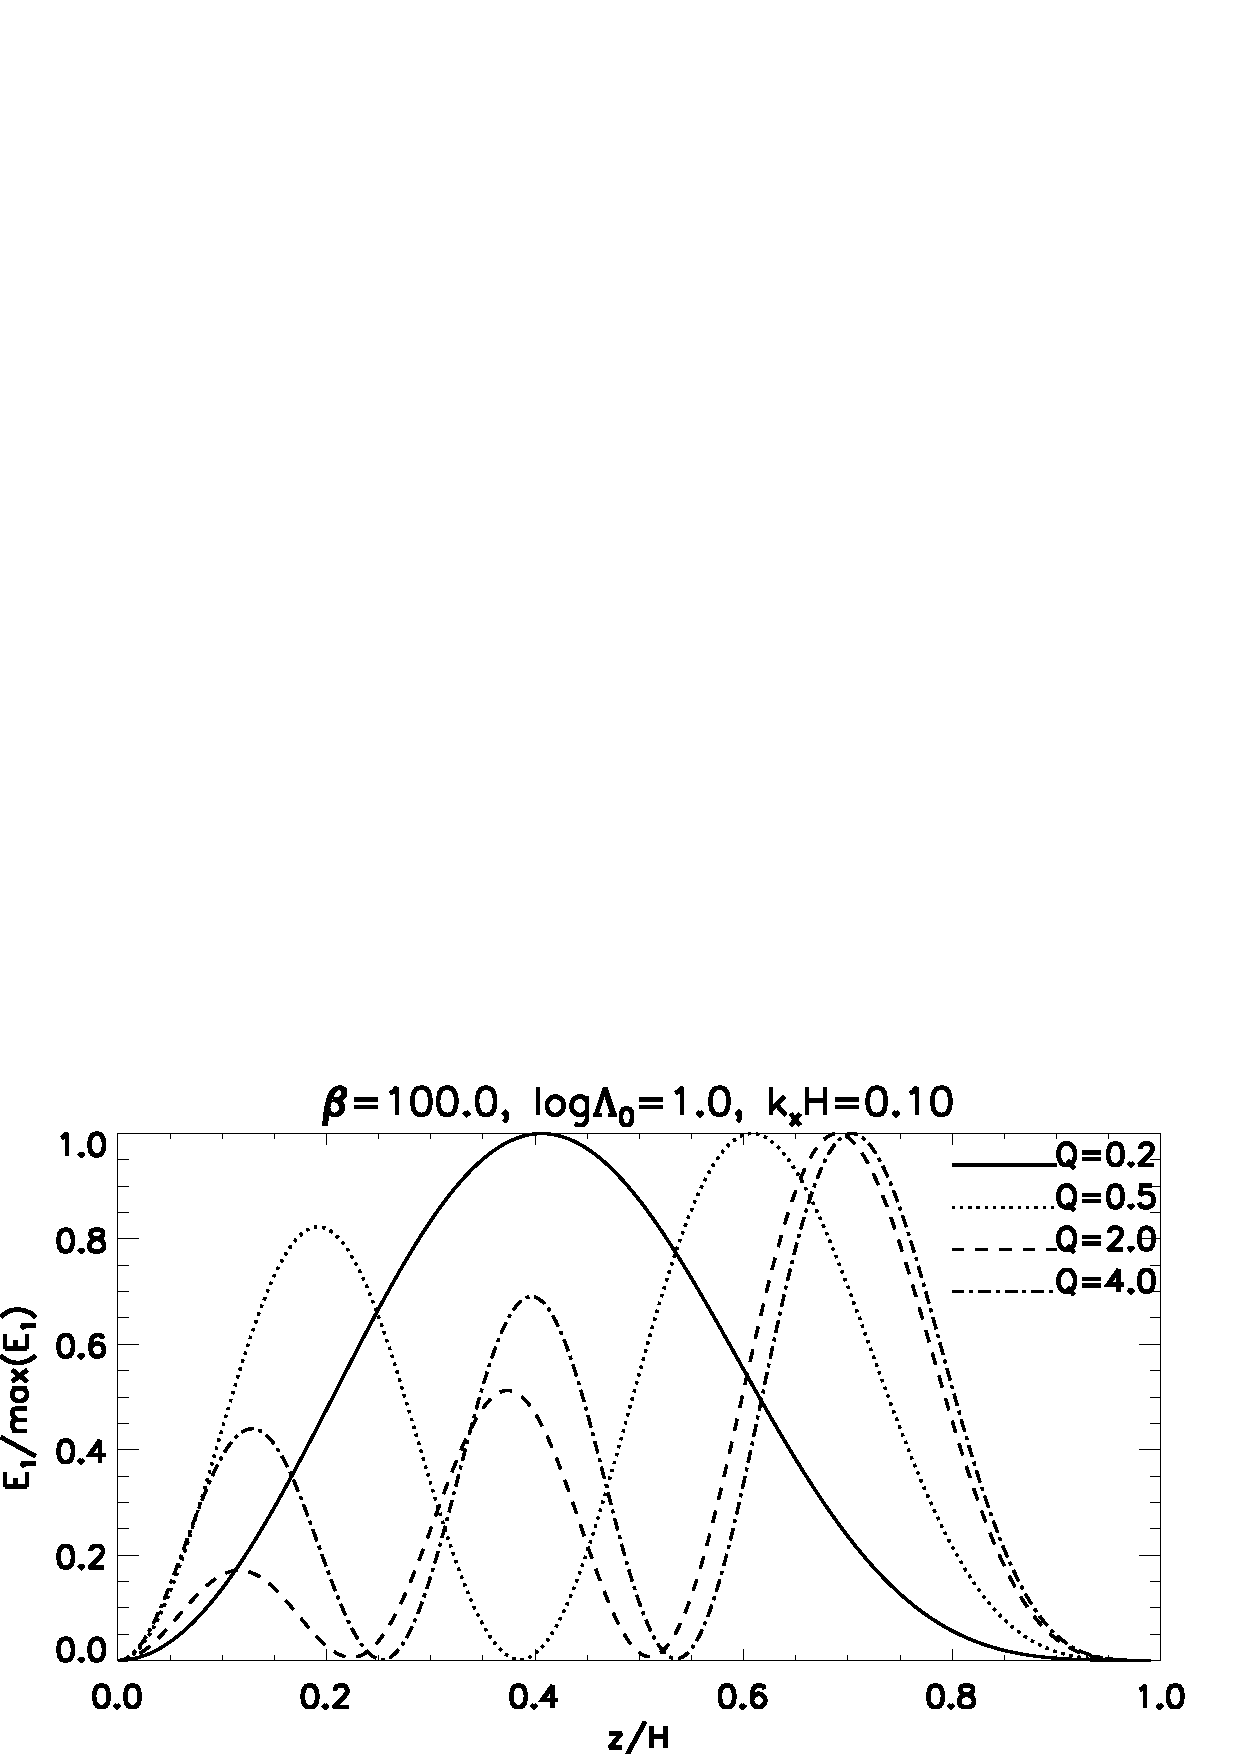
\includegraphics[width=\linewidth]{figures/compare_result_lambda10}
  \caption{Magnetic energies as a function of height, in the limit of
    ideal MHD, for various strengths of self-gravity.   
    \label{compare_result_lambda10}}
\end{figure}

Self-gravity appreciably decreases the MRI growth rates in the
resistive limit. Fig. \ref{lambda_poly_resis} plots 
Eq. \ref{sano_crit} for $\Lambda_0=0.3$. In the non-self-gravitating
disk ($Q=4$) the instability criterion is marginally satisfied and the
MRI operates. As $Q$ decreases, 
Eq. \ref{sano_crit} is violated and the MRI growth rate is
significantly reduced. This is seen for $Q=0.2$ where $\lambda \geq 2H$ throughout
the disk. (The instability is not completely surpressed since
Eq. \ref{sano_crit} is only an approximation.) Although the function
$f$ does not change significantly for the range of $Q$ considered, the
dependence of $\lambda_\mathrm{resis}$ on $f$ (and therefore $Q$) is
amplified by the denominator $\Lambda_0<1$ in the resistive case. For
resistive cases we find no nodes in the magnetic energy $E_1$ except
at end points, i.e. only the longest wavelength survives.   

\begin{figure}
  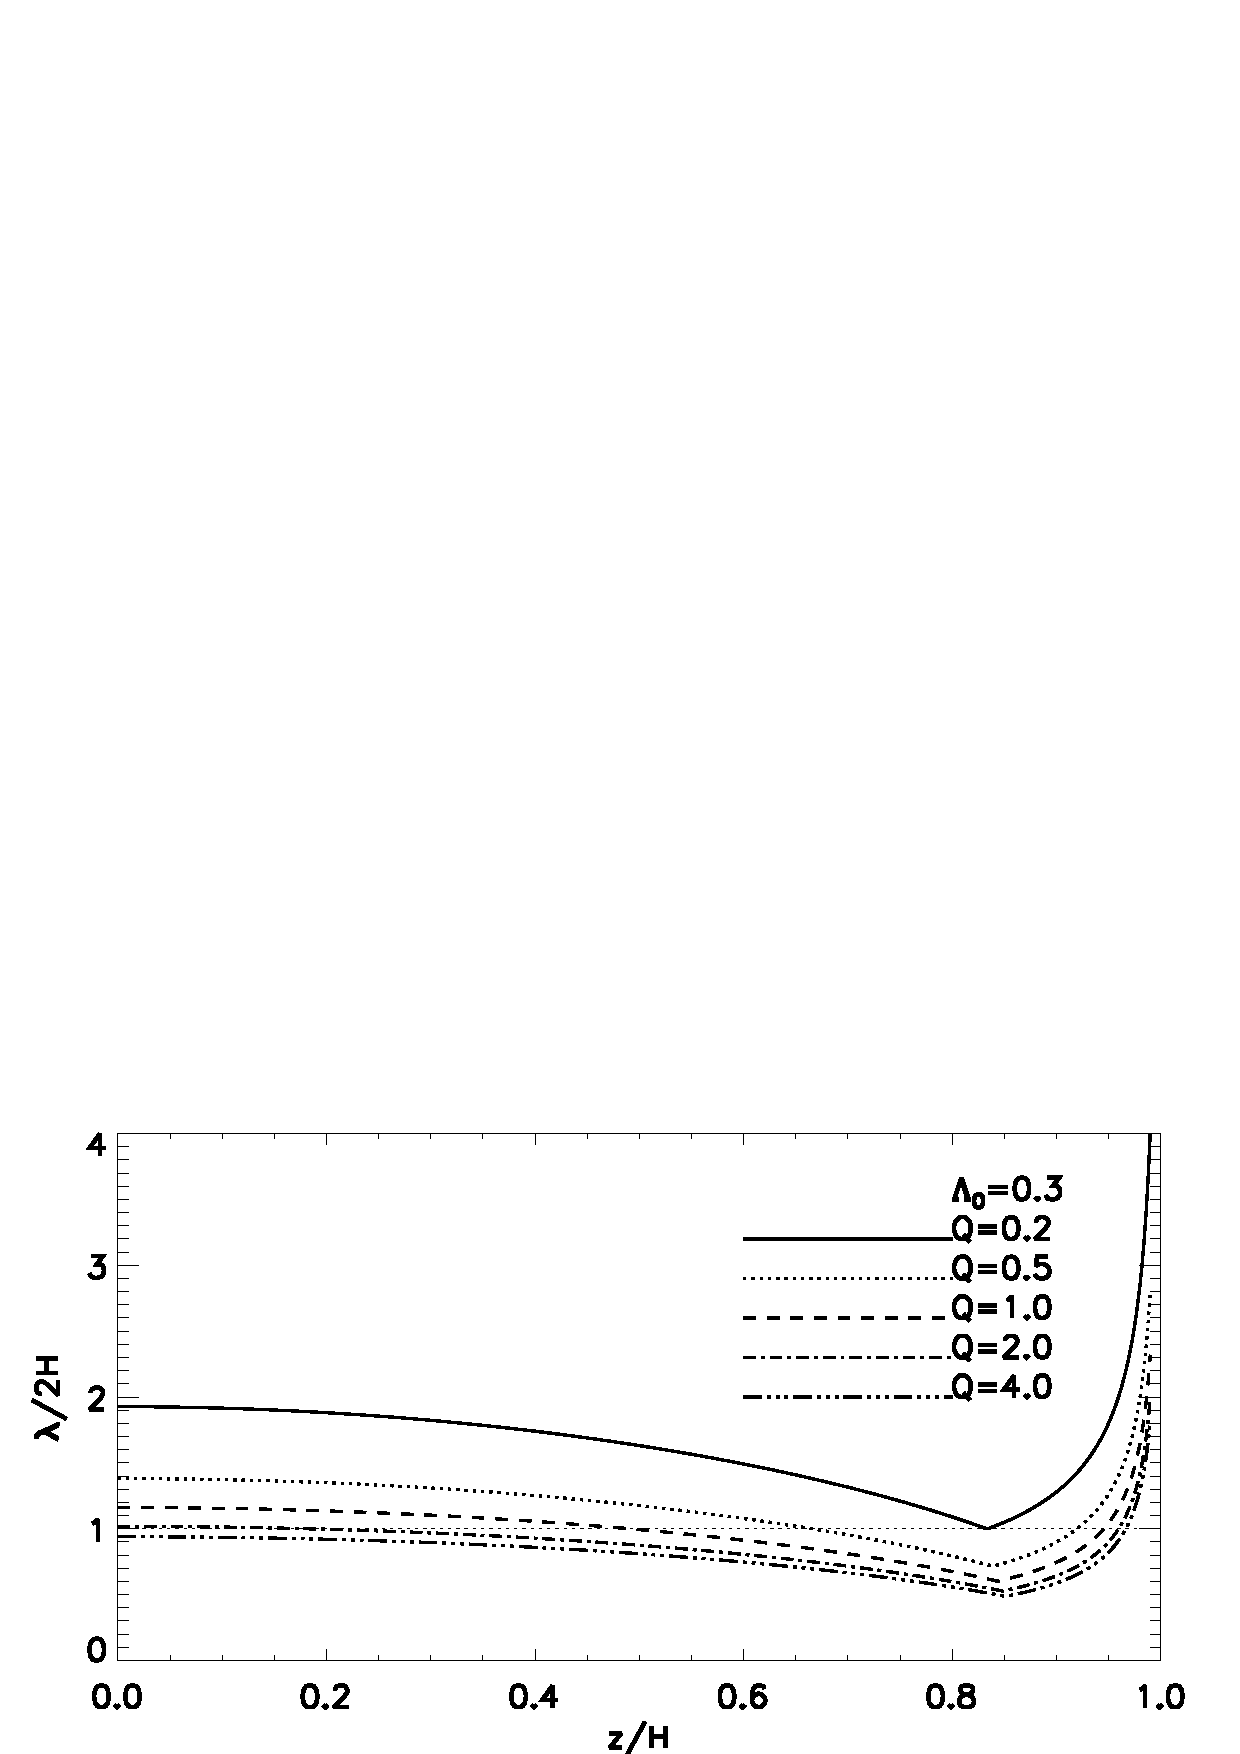
\includegraphics[width=\linewidth]{figures/lambda_poly_uniresis}
  \caption{Approximate wavelengths of the most unstable resistive MRI modes as given by
    Eq. \ref{sano_crit}---\ref{lambda_resis}, normalized by the 
    disk thickness, as a function of height for a range of Toomre $Q$
    values.  
    \label{lambda_poly_resis}}
\end{figure}

\subsubsection{Layered
  resistivity} 
Here we consider disks with mid-plane Elsasser number $\Lambda_0=0.1$
and a variable resistivity profile with
$A=10^2$. Fig. \ref{poly_layer} compares the magnetic  
energies for $Q=0.2,\,1$ and $4$. They have similar growth rates, $\gamma/\Omega
= 0.53,\,0.64$ and $0.66$, respectively. In the non-self-gravitating
limit ($Q=4$), the MRI is effectively surpressed for
$z\lesssim0.5H$. This is consistent with layered accretion. However,
in the massive disk ($Q=0.2$) the mode occupies a wider vertical
extent because its wavelength (in units of $H$) is larger. This
suggests that in massive disks the MRI is not well localized to the
active layer, as the instability takes on a more global character
compared to non-self-gravitating disks.        
%d is not as well localized

\begin{figure}
  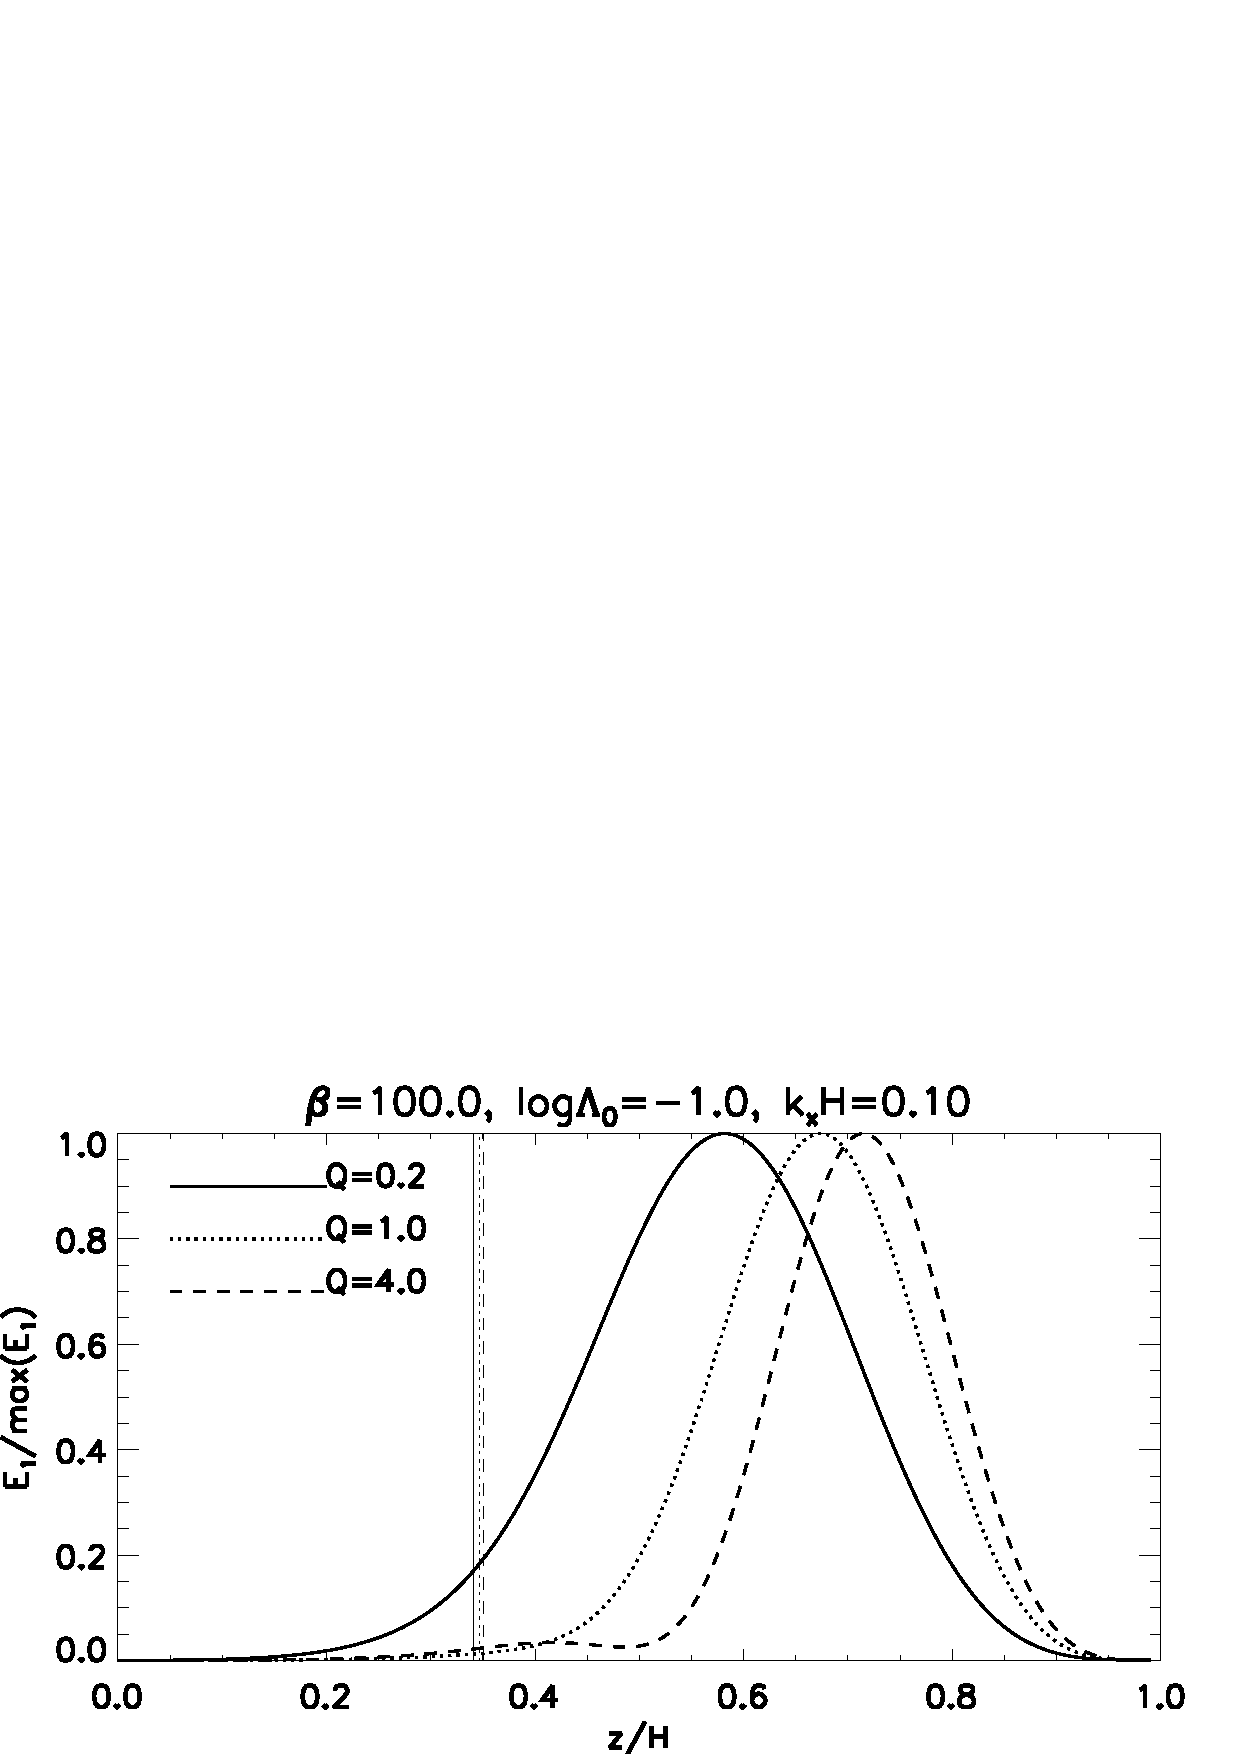
\includegraphics[width=\linewidth]{figures/compare_results_poly_layer_amp100}
  \caption{Magnetic energies as a function of height, for layered polytropic disks with
    such that the conductivity increases by a 
    factor of $10^2$ in going from the mid-plane to the upper disk
    boundary. The vertical lines indicate $\Lambda=1$ for each value
    of $Q$.
    \label{poly_layer}}
\end{figure}


\subsection{Influence of self-gravity on the MRI through the linear
  response}  
 
Our goal here is to examine whether or not self-gravity can amplify
the density perturbations caused by the MRI. We choose a massive 
isothermal disk with $Q=0.2$, which is still expected to be marginally
stable to gravitational instability \citep[][who find
a critical value of  $Q\simeq 0.2$]{mamat10}.  
The upper disk boundary is set to $Z_s=H$. The field is vertical.  

%resolution Nz=256

\subsubsection{Ideal case}
We first consider the limit of ideal MHD by adopting a uniform
resistivity with $\Lambda_0=100$. %Non-zero density perturbations
%require $k_x\neq0$ so we consider linear modes as a function of $k_x$.   



\begin{figure}
  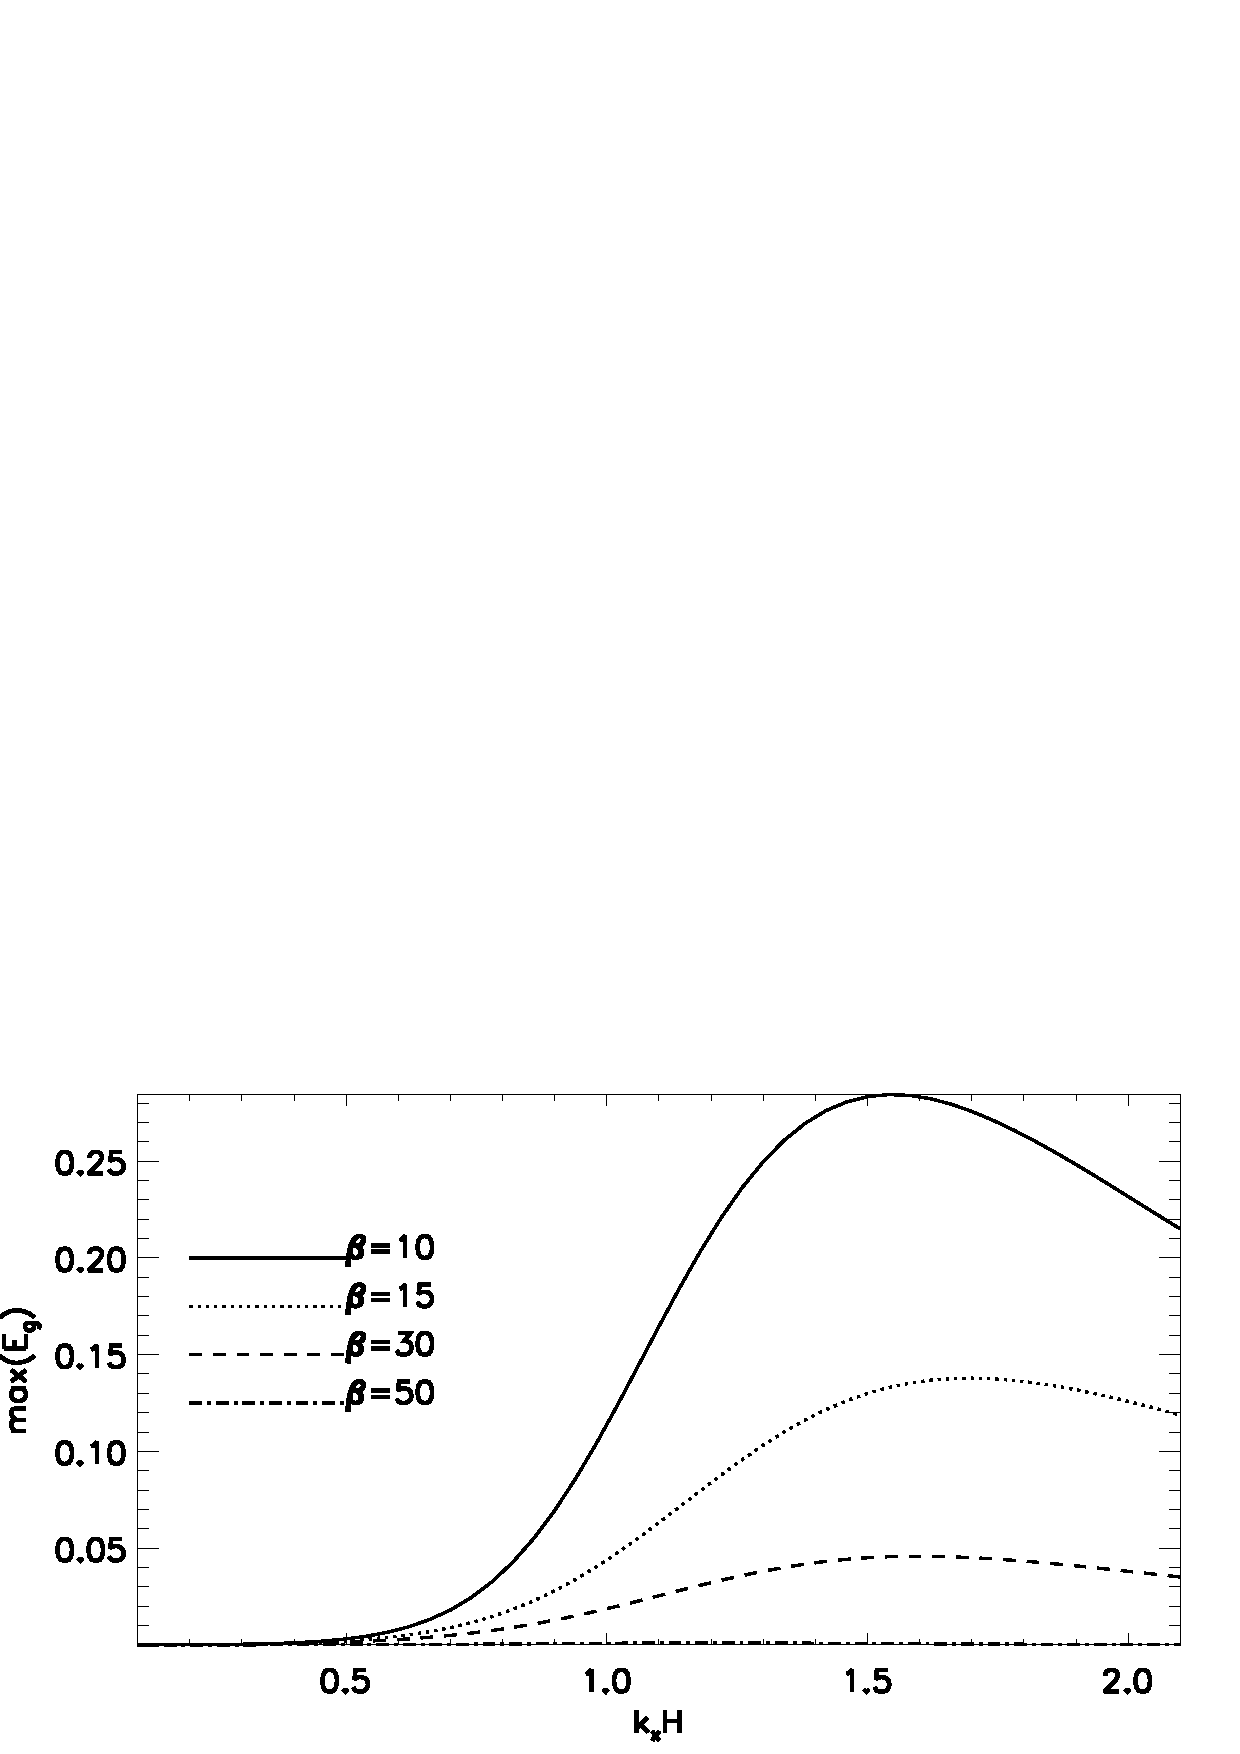
\includegraphics[width=\linewidth]{figures/compare_energy_ideal}
  \caption{Maximum gravitational potential energy perturbation
    associated with the MRI in a self-gravitating disk with $Q=0.2$ in
    the limit of ideal MHD ($\Lambda_0=10^2$). 
    \label{gravity_energy}}
\end{figure}





\subsubsection{Qualitative interpretation} 
In order to make sense of the above results, we consider ideal MHD and
a vertical field. For this discussion we will ignore stratification
and set $d/dz\to \imgi k_z$ where $k_z$ is a vertical 
wavenumber. Equivalently, we are considering regions close to the disk
midplane. The governing equations are then

\begin{align}
  &  0= v_A^2k^2\dvx + \imgi\sigma\left(\imgi\sigma \dvx - 2\Omega\dvy + \imgi k_x \w\right),\label{simp1}\\
  &  0= v_A^2k_z^2\left(\dvy + \frac{\imgi S
  }{\sigma}\dvx\right) + \imgi\sigma\left(\imgi\sigma\dvy +
  \frac{\kappa^2}{2\Omega}\dvx\right),\\
  & 0 = -k_z^2\w + \frac{\sigma^2}{c_s^2}W + \sigma k_x \dvx, \label{simp3}\\
  & 0 = k^2\dphi + \frac{\Omega^2}{c_s^2Q}W,\label{simp4}
\end{align}
where $k^2 = k_z^2 + k_x^2$. 

We imagine an iterative procedure to solve the above equations,
starting from the \emph{Cowling approximation}, defined to be the
solution to Eq. \ref{simp1}---\ref{simp3} with potential perturbation
set to zero. This is the standard MRI and we denote the solution as
$\dvx^{(0)}$, $\dvy^{(0)}$ and $W^{(0)}$. 

We now include self-gravity. In general, the MRI will have some
density perturbation so $W^{(0)}\neq0$. The Poisson equation implies
an associated potential perturbation,    
\begin{align} 
  \dphi = -\frac{\Omega^2}{c_s^2 Q k^2} W^{(0)}.
\end{align}
Physically, we expect $k^2\geq0$, so that a positive (negative) density
perturbation causes a negative (positive) potential perturbation. We
then regard $\dphi$ to alter the Cowling solution, so
that $\dvx^{0} \to \dvx^{0} + \dvx^{(1)}$ and similarly for $\dvy$ and
$W$. Then 
\begin{align}
  &   k_x\sigma \dphi = v_A^2k^2\dvx^{(1)} + \imgi\sigma\left[\imgi\sigma
  \dvx^{(1)} - 2\Omega\dvy^{(1)} + \imgi k_x W^{(1)}\right], \label{simp_pert1}\\ 
  &  0= v_A^2k_z^2\left[\dvy^{(1)} + \frac{\imgi S
    }{\sigma}\dvx^{(1)}\right] + \imgi\sigma\left[\imgi\sigma\dvy^{(1)} +
  \frac{\kappa^2}{2\Omega}\dvx^{(1)}\right],\label{simp_pert2}\\
  & k_z^2\dphi  = \left(\frac{\sigma^2}{c_s^2}-k_z^2\right)W^{(1)} +
  \sigma k_x \dvx^{(1)}.\label{simp_pert3} 
\end{align}
Now, if the perturbations to the magnetic field remain
unchanged, i.e. the mode remains close to the standard MRI, then
$\dvx^{(1)} \sim 0$ and $\dvy^{(1)}\sim0$, so Eq. \ref{simp_pert2} is
satisfied. Eq. \ref{simp_pert1} then require $\dphi +
W^{(1)}\sim0$. This is compatible with Eq. \ref{simp_pert3} if 
\begin{align}
  \left|k_z^2\right| \gg \left|\frac{\sigma^2}{c_s^2}\right|. \label{cond}
\end{align}
These assumptions imply
\begin{align}
  W^{(1)} \sim \frac{\Omega^2}{c_s^2 Q k^2} W^{(0)},\label{feedback}
\end{align} 
which indicates a non-zero density perturbation due to the
MRI can be amplified by self-gravity. 
%However, the magnetic field
%perturbations remain that in the   

By introducing $\hat{k}_z=k_zH$, Eq. \ref{cond} can be
non-dimensionalized to 
\begin{align}
  \left|\frac{\hat{\sigma}^2}{f^2\hat{c}_s^2\hat{k}_z^2}\right|\ll 1.  
\end{align}


%\begin{align}
%  
%\end{align}
%However, in the full problem $\dphi$ appears in the $\mathcal{G}$

%We write the horizontal velocities and enthalpy perturbations as
%\begin{align}
%  \dvx &= u + \Delta u,\\
%  \dvy &= v + \Delta v,\\
%  W    &= w + \Delta w,
%\end{align}
%where $u$, $v$ and $w$ is the solution to
%Eq. \ref{simp1}---\ref{simp4} in the Cowling approximation, in which
%the Poisson equation is ignored and the potential perturbation set to
%zero. 
